\documentclass{beamer}

\usepackage{graphicx}
\usepackage{textpos}
\usepackage{listings}
\usepackage{tikz}
\usepackage{listofitems}

\definecolor{codegreen}{rgb}{0,0.6,0}
\definecolor{codegray}{rgb}{0.5,0.5,0.5}
\definecolor{codepurple}{rgb}{0.58,0,0.82}
\definecolor{backcolour}{rgb}{0.95,0.95,0.92}

\lstdefinestyle{python}{
  backgroundcolor=\color{backcolour},   
  commentstyle=\color{codegreen},
  keywordstyle=\color{magenta},
  numberstyle=\tiny\color{codegray},
  stringstyle=\color{codepurple},
  basicstyle=\ttfamily\footnotesize,
  breakatwhitespace=false,         
  %breaklines=true,                 
  captionpos=b,                    
  keepspaces=true,                 
  %numbers=left,                    
  %numbersep=5pt,                  
  showspaces=false,                
  showstringspaces=false,
  showtabs=false,                  
  tabsize=2
}

\lstset{style=python}

\usetheme{Madrid}
\useoutertheme{miniframes} % Alternatively: miniframes, infolines, split

% Setup the university's color pallette
\definecolor{UIUCorange}{RGB}{19, 41, 75} 
\definecolor{UIUCblue}{RGB}{232, 74, 39} 


\setbeamercolor{palette primary}{bg=UIUCorange,fg=white}
\setbeamercolor{palette secondary}{bg=UIUCblue,fg=white}
\setbeamercolor{palette tertiary}{bg=UIUCblue,fg=white}
\setbeamercolor{palette quaternary}{bg=UIUCblue,fg=white}
\setbeamercolor{structure}{fg=UIUCorange} % itemize, enumerate, etc
\setbeamercolor{section in toc}{fg=UIUCblue} % TOC sections

\setbeamercolor{subsection in head/foot}{bg=UIUCorange,fg=UIUCblue}
\setbeamercolor{subsection in head/foot}{bg=UIUCorange,fg=UIUCblue}

\usepackage[utf8]{inputenc}
\usepackage{graphicx}


%Information to be included in the title page:
\title{\textbf{Introduction to the Course - Part 1}}
\author{\textbf{David H Smith IV}}
\institute[\textbf{UIUC}]{\textbf{University of Illinois Urbana-Champaign}}
\date{\textbf{Tuesday, Aug 17 2021}}

\setbeamertemplate{title page}[default][colsep=-4bp,rounded=true]
\addtobeamertemplate{title page}{\vspace{3\baselineskip}}{}
\addtobeamertemplate{title page}{
  \begin{textblock*}{\paperwidth}(-1.0em, -1.2em)
    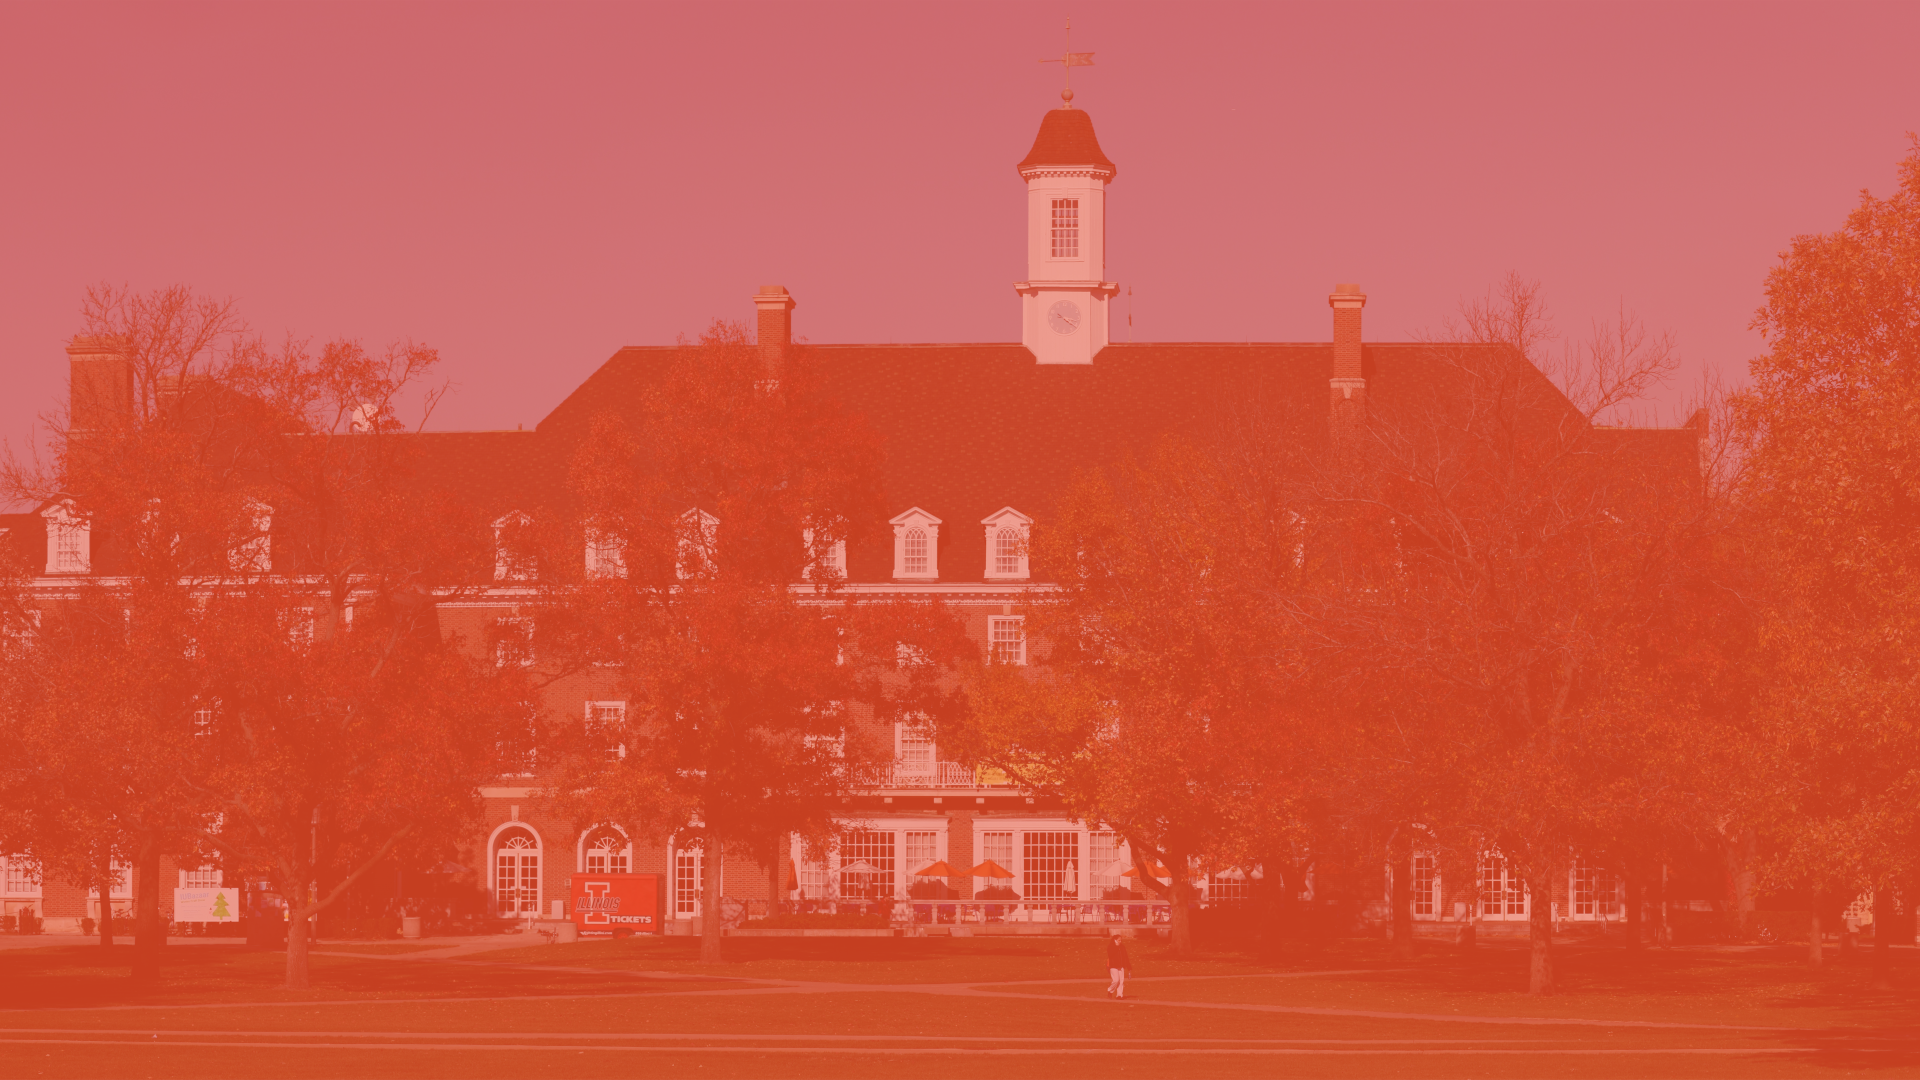
\includegraphics[width=\paperwidth, height=\paperheight]{imgs/uiuc.png}
  \end{textblock*} 
}{}

\begin{document}

\frame{\titlepage}

\section{Course Overview}

\begin{frame}
  \frametitle{Course Outcomes}
  \begin{itemize}
    \item Given a small section of code you should be able to:
      \begin{itemize}
        \item Trace through and predict it's output.
        \item Describe, in plain English, what it does.
      \end{itemize}
    \item Write a small python program some using the fundamentals you will learn in this course.
    \item Version control with Git and GitHub
    \item Other side topics as time allows (e.g, the internet)
  \end{itemize}
\end{frame}

\begin{frame}
  \frametitle{Lecture Time}
  \begin{itemize}
    \item We ask multiple choice questions through the following process:
      \begin{enumerate}
        \item You answer the poll individually, for participation points.
        \item Then you discuss with your peers in your assigned lecture discord group.
        \item You will answer the poll a second time for, credit.
      \end{enumerate}
      \\ \vfill 
    \item These will use ABCD cards:\\
      \begin{minipage}{0.45\textwidth}
        \begin{itemize}
          \item Apps are listed on the course website: 
          \item Physical copies are avaliable if you would prefer.
        \end{itemize}
      \end{minipage}
      \begin{minipage}{0.45\textwidth} 
        
\includegraphics[height=75px]{./imgs/abcd.png}
      \end{minipage}
  \end{itemize}
\end{frame}

\begin{frame}
  \frametitle{Discord}
  \begin{itemize}
    \item \textbf{Invite link:} https://discord.gg/sADNwpX4
    \item Where office hours are posted.
    \item Please feel free to ping me in the group text channel if you have any questions by `@ing' me.
    \item Feel free to use the group discussion rooms to talk about homework and ping me if you get stuck. 
    \item Please only message me or ping me through the public chat. Do not direct message me.
  \end{itemize}
\end{frame}

\begin{frame}
  \frametitle{zyBooks \& Post Readings}
  \begin{itemize}
    \item zyBooks Participation and Challenge Activities:
    \begin{itemize}
      \item Two participation activities due a week (usually).
      \item Challenge activities due every Sunday (again usually).
      \item Always defer to the course calender and the dates listed on the assignment in zyBooks.
    \end{itemize}
    \item PrairieLearn Post Readings
    \begin{itemize}
      \item Due with every reading activity
      \item \textbf{Muddiest Points: } What point did you find most confusing. If nothing, what do you think others found the most confusing?
      \item \textbf{Future Detail: } What would you like to be covered more in depth during lecture?
      \item \textbf{Time Spent: } How long did you spend doing the reading?
    \end{itemize}
  \end{itemize}
\end{frame}

\begin{frame}
  \frametitle{Weekly Schedule}
  \begin{itemize}
    \item General weekly schedule: https://hamiltonfour.tech/uni-high-fall-21/schedule/
    \item Item specific schedule: https://hamiltonfour.tech/uni-high-fall-21/calendar/
  \end{itemize}
\end{frame}

\begin{frame}
  \frametitle{First poll question! - Getting Help}
  \begin{enumerate}
    \item You must do all of your homework alone (not even I can help)
    \item You can get any help you want as long as you type in the answers.
    \item Students can only discuss the homework at a high level; code must not be shown to other students, but you can as TAs for help.
    \item Homework can be done in groups of two students.
  \end{enumerate}
\end{frame}

\begin{frame}
  \frametitle{Due this Thursday}
  \begin{enumerate}
    \item Look over and get familiar with the course website. 
    \item Get Discord setup.
    \item Topic 1 reading and participation activities
      \begin{itemize}
        \item Cover half of the topics today and the rest tommorow.
        \item Read the following chapters just for information: 1.[5-8]
        \item Read the following chapters for comprehension: 1.[1-4], 1.9
      \end{itemize}
    \item Wednesday is a history lesson
    \item Thursday we'll start diving into Python.
  \end{enumerate}
\end{frame}


\end{document}
